\begin{titreTice}[Géométrie dans l'espace]

\Titre{Construction et visualisation}{4}
\end{titreTice}


\begin{CpsCol}
\textbf{Construction et visualisation}
\begin{description}
\item[$\square$] Construire avec un logiciel dynamique un solide usuel
\end{description}
\end{CpsCol}

\subsection*{Construction d'un cube }

\begin{enumerate}
\item Ouvrir une fenêtre 2D et une fenêtre 3D
\item Placer 2 points A et B dans la fenêtre 2D 
\item A l'aide de l'icône \textbf{Polygone régulier} 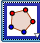
\includegraphics[scale=0.4]{poly.jpg}, construire un carré ABCD.
\item Sélectionner la fenêtre 3D. Une barre, d'icônes propre 3D s'initialise à la place de la barre d'icônes 2D. 

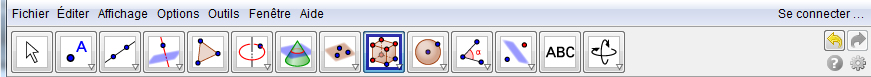
\includegraphics[scale=0.5]{outils-3D.jpg} 

\item Utiliser l'icône 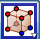
\includegraphics[scale=0.5]{cube.jpg} pour extruder le cube. Cliquer sur les points $A$ et $B$ dans la fenêtre 3D. Et voilà le cube.

On peut placer directement 2 points dans la \textbf{fenêtre 3D }et créer un cube mais si l'on souhaite un cube "posé", il est préférable d'utiliser cette méthode.

\end{enumerate}

\subsection*{Construction d'un plan }

Un plan passe par 3 points non alignés.

 A l'aide de l'icône \textbf{Plan passant par 3 points} 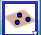
\includegraphics[scale=0.4]{plan.jpg}, construire le plan ABE.
 
\textbf{Attention}, les points induits de la construction du solide construit précédemment ne sont pas sélectionnables \mbox{directement}. Il faut les sélectionner dans la fenêtre \textbf{Algèbre}.













